\documentclass[10pt,a4paper]{article}
\usepackage[utf8]{inputenc}
\usepackage[english]{babel}
\usepackage{amsmath}
\usepackage{amsfonts}
\usepackage{amssymb}
\usepackage{graphicx}
\usepackage[left=3.5cm,right=3.5cm,top=3cm,bottom=3cm]{geometry}
\author{Fabian Schubert}
\title{Driven Random Dynamic Reservoir with Homeostatic Variance Control}

%\def\avgt#1{\langle {#1} \rangle_T}
%\def\avgp#1{\langle {#1} \rangle_P}

\newcommand{\avgt}[1]{\left< #1 \right>_T}
\newcommand{\avgp}[1]{\left< #1 \right>_P}

\parskip=5pt

\begin{document}
\begin{center}
\begin{LARGE}
\textbf{Driven Random Dynamic Reservoir with Homeostatic Variance Control}\\
\end{LARGE}
\end{center}

\section{Model Description}

\subsection{Dynamics}
\begin{align}
x_i^{t+1} &= \mathrm{tanh}\left( g_i^t I_i^{t+1} \right) \\
I_i^{t+1} &= \sum_{j=1}^{N_{\rm net}} W_{ij} x_j^t + E_i^{t+1} \\
g_i^{t+1} &= \mu_{g} \left[ \sigma_{\rm target}^2 - \left( x_i^t - \langle x_i \rangle \right)^2 \right]
\end{align}

\subsection{Parameters / Settings}

$W_{ij}$ is a sparse random matrix with connection probability ${\rm cf_{net}}$. Nonzero entries were drawn from a Gaussian distribution $\mathcal{N}(\mu = 0,\sigma = \sigma_{\rm conn} / \sqrt{N_{\rm net} {\rm cf_{net}}})$. Diagonal entries were always set to zero.

$E^t_{i}$ are random vectors of size $N_{\rm net}$ with independent entries drawn from a Gaussian distribution $\mathcal{N}(\mu = 0,\sigma = \sigma_{\rm ext})$. External input is turned off after $t_{\rm ext.off}$.

By changing individual gain values $g_i$, the homeostatic control tries to drive the activity standard deviation of every cell to the value given by $\sigma_{\rm target}$. However, this mechanism is also switched off after $t_{\rm ext.off}$. This is done because we can assume that homeostatic processes would biologically act on much slower timescales than changes in input. Before $t_{\rm ext.off}$, we can set $\mu_{g}$ to relatively high values to let homeostasis converge under external drive.

See all parameters in Table \ref{tab:params}.
\begin{table}[h]
\caption{Model Parameters}
\centering
\vspace{5pt}
\begin{tabular}{l | r}
\textbf{Parameter} & \textbf{Value} \\
\hline
$N_{\rm net}$           & 500\\
${\rm cf_{net}}$        & 0.1\\
$\sigma_{\rm conn}$     & 1.0\\
$\sigma_{\rm ext}$		& 1.0\\
$\mu_{g}$               & 0.0005\\
$\sigma_{\rm target}$ 	& 0.33\\
$n_t$ (Sim. Steps)      & 200000\\
$t_{\rm ext.off}$       & 100000
\end{tabular}
\label{tab:params}
\end{table}
\newpage
\section{Results}
Exemplary results are shown in Fig. \ref{fig:ex_results}.

\begin{figure}[h]
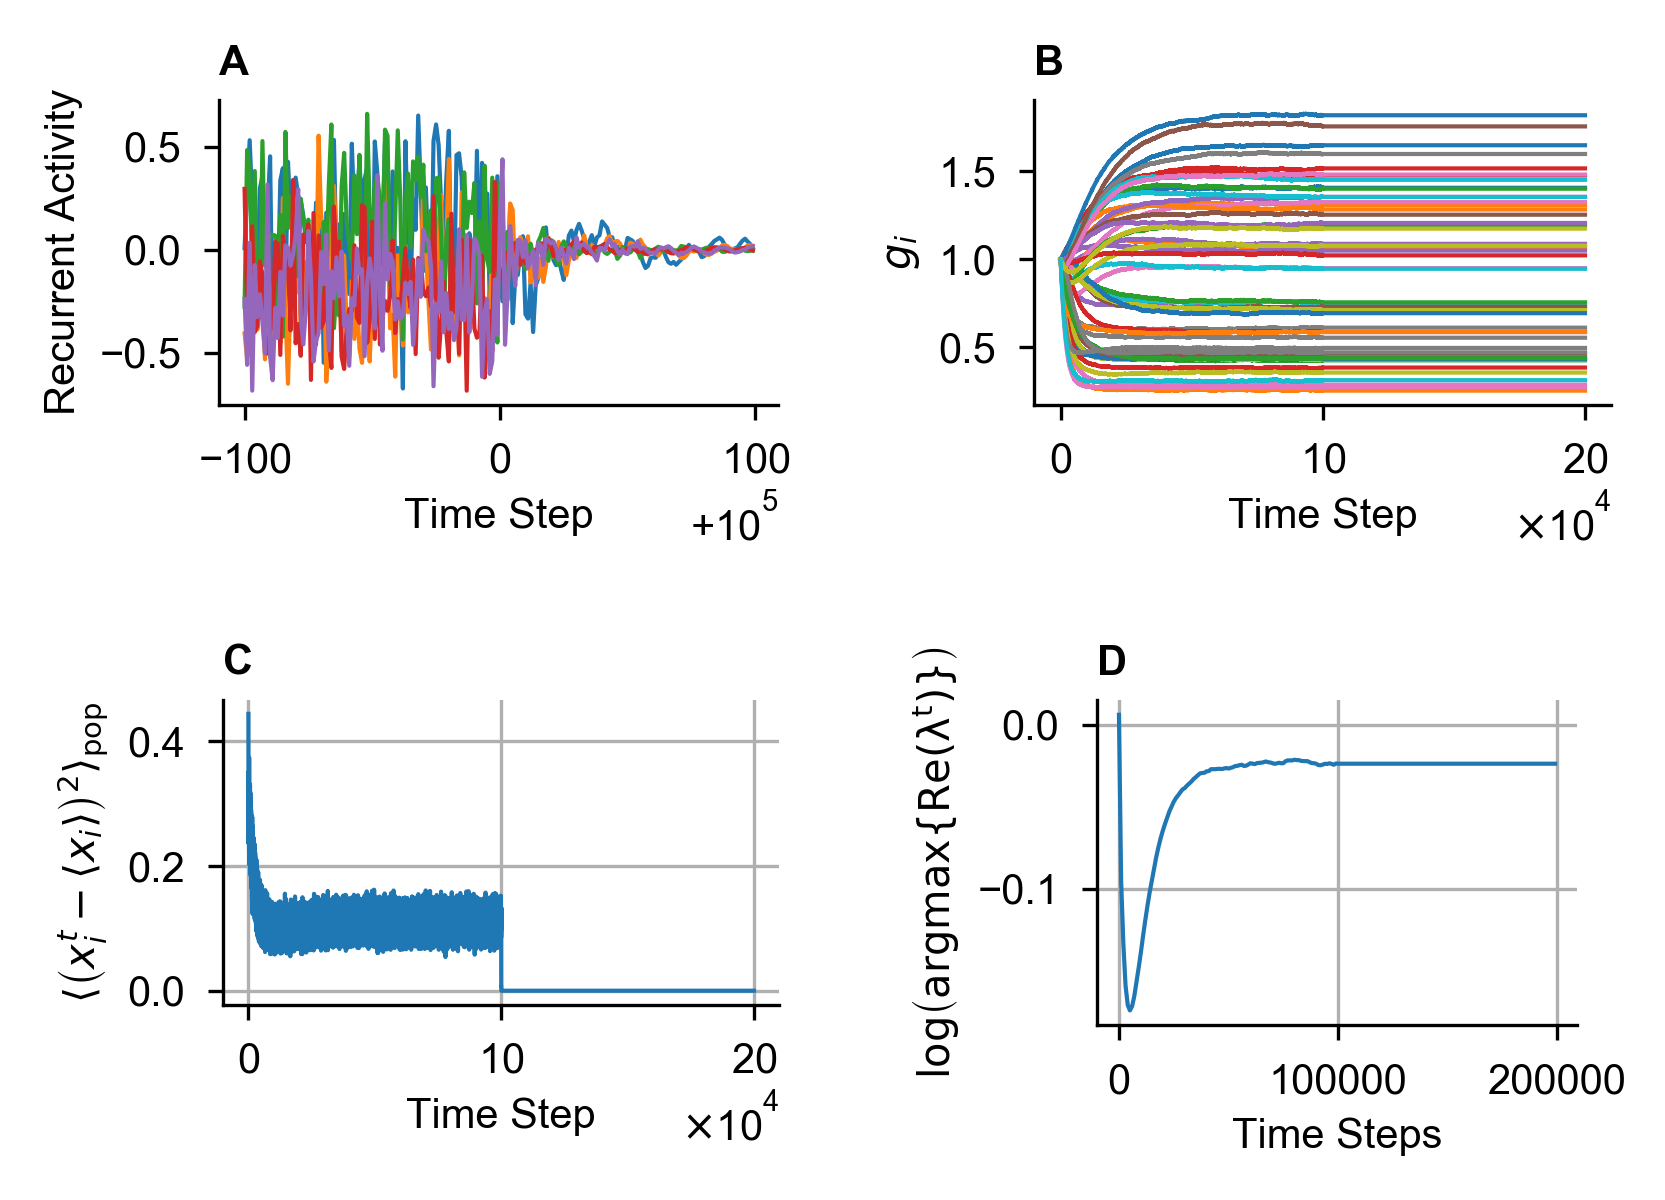
\includegraphics[width=\textwidth]{../plots/im_comp.png}
\caption{{\bf A}: Sample of activity within $\left[ t_{\rm ext.off} - 100, t_{\rm ext.off} + 100 \right]$. {\bf B}: Gain dynamics of $N_{\rm net}/10$ exemplary neurons. {\bf C}: Population mean of squared activity. {\bf D}: Log. of largest real part of eigenvalues of $g_i^t W_{ij} $.{\bf E}: Sample of population activity for the last 100 steps.}
\label{fig:ex_results}
\end{figure}

\section{Mean Field Approximation}

We would like to find an approximate relation between the gain resulting from homeostasis and the input and target variance. In the following, we shall denote by $\avgt{\cdot}$ an average over time and by $\avgp{\cdot}$ over the population. If we linearize the neural activation function and take an average over time, we get
\begin{align}
	\avgt{x_i^2} &= g_i^2 \avgt{\left(\sum_{j=1}^{N_{\rm net}} W_{ij} x_j + E_i\right)^2} \\
	&= g_i^2 \avgt{\left( \sum_{j=1}^{N_{\rm net}} W_{ij} x_j \right)^2} + g_i^2 E_i^2 \\
	&= g_i^2 \sum_{j,k=1}^{N_{\rm net}} W_{ij}W_{ik} \avgt{x_j x_k} + g_i^2 E_i^2 \; .
\end{align}
If we assume that the system is in a chaotic state we can set $\avgt{x_j x_k}=0$ for $j\neq k$. This leads to
\begin{equation}
	\avgt{x_i^2} = g_i^2 \left( \sum_{j=1}^{N_{\rm net}} W_{ij}^2 \avgt{x_j^2} + \sigma_{\rm ext}^2 \right)
\end{equation}
where we have assumed $\avgt{E_i} = 0$ for all $i$.

By design, our homeostatic mechanism fixes all $\avgt{x_i^2}$ to $\sigma_{\rm target}^2$. Thus,
\begin{align}
	\sigma_{\rm target}^2 &= g_i^2 \left( \sigma_{\rm target}^2 \sum_{j=1}^{N_{\rm net}} W_{ij}^2 + \sigma_{\rm ext}^2 \right) \\
	g_i &= \left(\sum_{j=1}^{N_{\rm net}} W_{ij}^2 + \sigma_{\rm ext}^2 / \sigma_{\rm target}^2\right)^{-1/2} \; .
\end{align}

Since $W_{ij}$ is a random Gaussian matrix with variance $\sigma_{\rm conn}^2/\left( N_{\rm net} cf_{\rm net} \right)$ , $\sum_{j=1}^{N_{\rm net}} W_{ij}^2$ follows a $\chi^2$ - distribution with variance $\frac{2N_{\rm net} cf_{\rm net} \sigma_{\rm conn}^2}{N_{\rm net}^2 cf_{\rm net}^2} = \frac{2 \sigma_{\rm conn}^2}{N_{\rm net} cf_{\rm net}}$. For $N_{\rm net} \rightarrow \infty $, its variance vanishes and consequently, all $g_i$ converge to the same value, namely 
\begin{equation}
	g = \left(\sigma_{\rm conn}^2 + \sigma_{\rm ext}^2 / \sigma_{\rm target}^2\right)^{-1/2} \; . \label{eq:gain_pred}
\end{equation}
This equation predicts that $g$ should not change if the ratio between target and input variance remains constant. We ran a parameter sweep over $\sigma_{\rm ext}$ and $\sigma_{\rm target}$ with a network of $N_{\rm net} = 1000$ neurons and looked at the resulting distribution of gains and the maximal Lyapunov exponent. Importantly, this approximation suggests that the network should tune into a subcritical configuration for any non-vanishing external input. Even though this is not strictly verified in the numerical simulation, see Fig.~\ref{fig:gain_std_in_std_targ_sweep}A, it holds for the majority of $ \sigma_{\rm ext}$/$\sigma_{\rm target}$ combinations.
\begin{figure}
	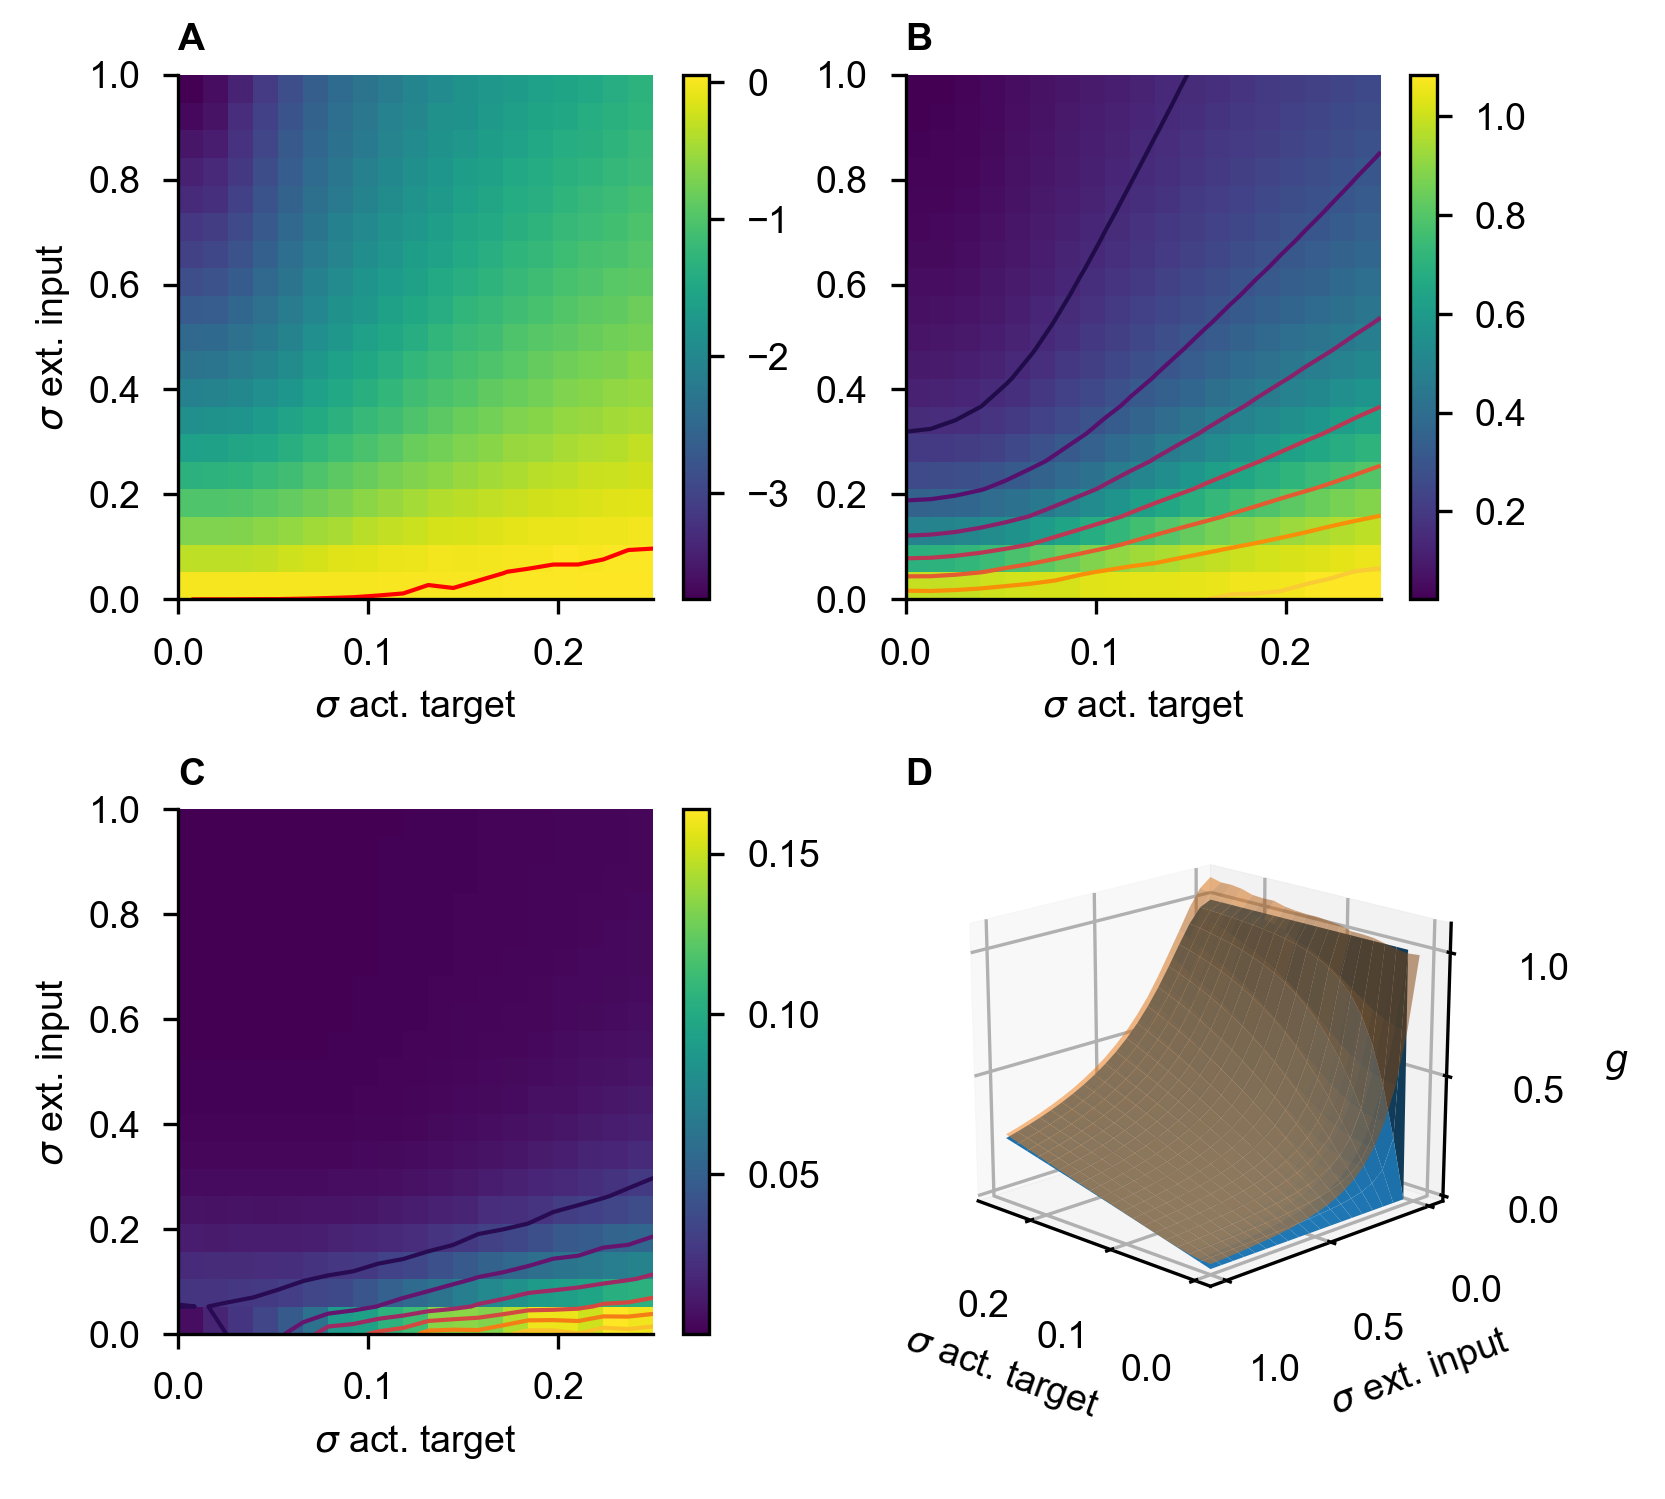
\includegraphics[width=\textwidth]{../plots/std_in_std_target_sweep_fig.png}
	\caption{Parameter sweep, run on a network with $N_{\rm net}=1000$. {\bf A}: Log of largest absolute value of eigenvalues of $g_i W_{ij}$. Red line marks the zero transition. {\bf B} : $\avgp{g_i}$. {\bf C}: $\avgp{(g_i - \avgp{g_i})^2}$ . {\bf D}: Prediction of \eqref{eq:gain_pred} (blue) vs. numerical result (orange) of $\avgp{g_i}$. }
	\label{fig:gain_std_in_std_targ_sweep}
\end{figure} 

\end{document}